
\documentclass[a4paper, 11pt]{article}
\usepackage[top=3cm, bottom=3cm, left = 2cm, right = 2cm]{geometry} 
\geometry{a4paper} 
\usepackage[utf8]{inputenc}
\usepackage{textcomp}
\usepackage{graphicx} 
\usepackage{amsmath,amssymb}  
\usepackage{bm}  
\usepackage[pdftex,bookmarks,colorlinks,breaklinks]{hyperref}  
\usepackage{memhfixc} 
\usepackage{float}
\usepackage{pdfsync}  
\usepackage{fancyhdr}
\pagestyle{fancy}
\fancyhead[R]{IIT BOMBAY}
\fancyhead[L]{
\includegraphics[width=3cm]{IITB.png}}
\begin{document}
\definecolor{darkblue}{RGB}{0, 0, 139}
\begin{center}
    {\fontsize{30}{32}\selectfont \textbf{Performance Report}}
\end{center}
\vspace{2cm}
{\fontsize{16}{18}\selectfont \textbf{Name : \color{darkblue}Aakash Gupta}}\\ %name
\newline
{\fontsize{16}{18}\selectfont \textbf{Roll Number : \color{darkblue}23b0953}} %roll number
\vspace{1cm}
\section{\fontsize{20}{22}\textbf{Attendance}}
{\fontsize{14}{16}\textit{\underline{\color{darkblue}Congratulations! Your attendance is 100.0\%}}}\\ 
\vspace{1cm}
\section{\fontsize{20}{22}\textbf{Marks}}
\vspace{2cm}
\begin{table}[!h]
    \centering
    \fontsize{18}{20}\selectfont
    \begin{tabular}{|p{5cm}|p{5cm}|}
    \hline
    \textbf{Examination} & \textbf{Marks} \\
    \hline
    \hline\\endsem & 8.39 \\
midsem & 15.38 \\
quiz1 & 32 \\
quiz2 & 6.37 \\
total & 62.14 \\
\hline
    \end{tabular}
\end{table}
\newpage
\vspace{3cm}
\section{\fontsize{20}{22}\textbf{Performance Index}}
\vspace{1cm}
{\fontsize{14}{16}\textit{\underline{Overall Grade : \color{darkblue}AP}}}\\
\newline
{\fontsize{14}{16}\textit{\underline{Current CPI : \color{darkblue}10}}}\\
\newline
{\fontsize{14}{16}\textit{\underline{Percentile : \color{darkblue}99.45945945945945}}}\\
\newline
{\fontsize{14}{16}\textit{\underline{Rank : \color{darkblue}2}}}\\
\newline
{\fontsize{14}{14}\textbf{Congratulations!You have been above average in all exams!}}\\
\begin{figure}
    \centering
    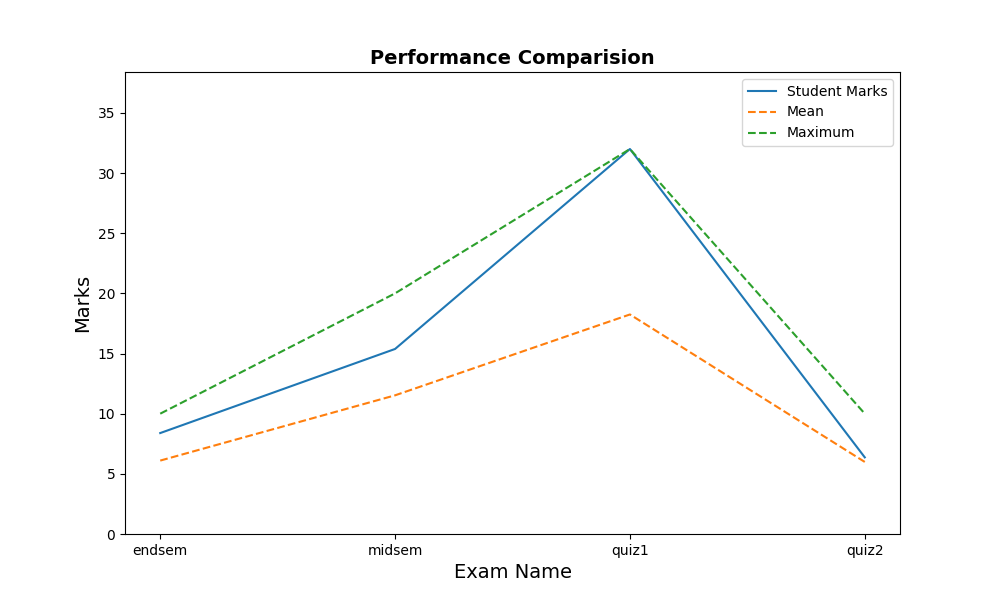
\includegraphics[width=12cm,height=12cm]{compare.png}
    \caption{\textbf{Relative Analysis}}
\end{figure}
\vspace{2cm}
\begin{flushright}
    {\fontsize{22}{22}\textit{\textbf{\color{darkblue}Thank You}}}
\end{flushright}
\end{document}